

\begin{figure}
    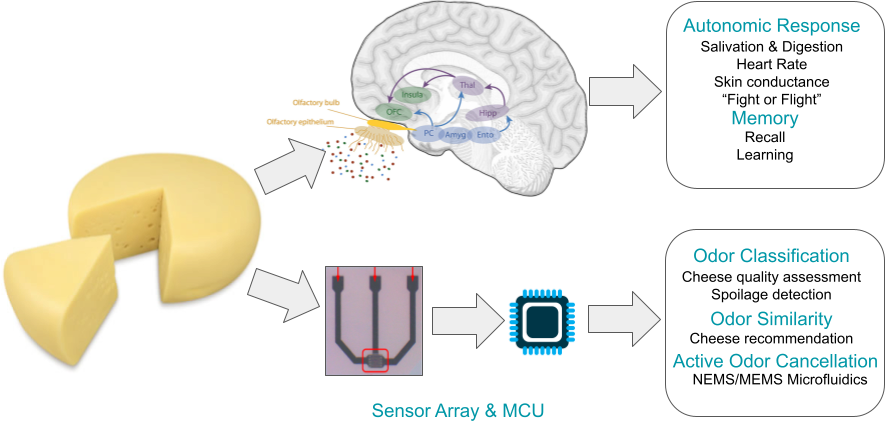
\includegraphics[width=\linewidth]{man_vs_machine.png}
    \caption{\small
        The human olfactory system transduces chemicals into electrical signals
        in the olfactory epithelium. Signals are then broadcast to a number of
        different parts of the brain, which enable autonomic nervous system
        responses, and can conjure memories and enable learning. This is
        mimicked in an odor sensor processor, where chemical sensor arrays
        transduce chemicals into odor signals which are sent to a compute
        element to execute odor related tasks.
    }
    \label{fig:man_vs_machine}
\end{figure}


Odor is a biological and psychological phenomenon (Figure~\ref{fig:man_vs_machine}) .  As such, chemical sensors
do not directly attempt to sense \textit{odors}, but rather to detect the
presence of \textit{chemical odorants}~\cite{dravnieks1985atlas,
snitz2019smellspace, keller2017predicting, malnic1999combinatorial}. A large
body of work has attempted to identify chemical-odor
relationships~\cite{snitz2019smellspace, keller2017predicting,
zhou2018hyperbolic, koulakov2011search, mamlouk2004dimensions}, e.g., 3-phenyl
propyl propionate has a `floral' odor, while (unsurprisingly) ethyl vanillin
has a `vanilla' odor~\cite{the_good_scents_company_2021}.  Thus, it is possible
to use chemical sensors to sense odors. Chemical sensors, such as metal-oxide
gas sensors, often operate on a basis of changes in electrical resistance in
reaction to the presence of one or more chemical analytes, with a higher
presence of the target analyte leading to larger changes in electrical
resistance.  However, these sensors are inherently noisy, as they will react to
the presence of chemicals suitably similar to their analyte (even if the
non-targeted chemical has a very different perceived odor).  Thus, a single
sensor is often inadequate for distinguishing between a quantity of its target
analyte, and a larger quantity of a non-target
analyte~\cite{schroeder2018carbon}. As such, commercial and academic
\textit{electric noses (e-nose)} use several sensors in a \textit{chemical
sensor array}.  The signals transduced by the sensor array is then fed into a
signal processing and/or machine learning algorithm in order to perform an
\olfc{} task, such as odor identification, odor pleasantness estimation, etc.

\begin{figure}[h]
    \centering
    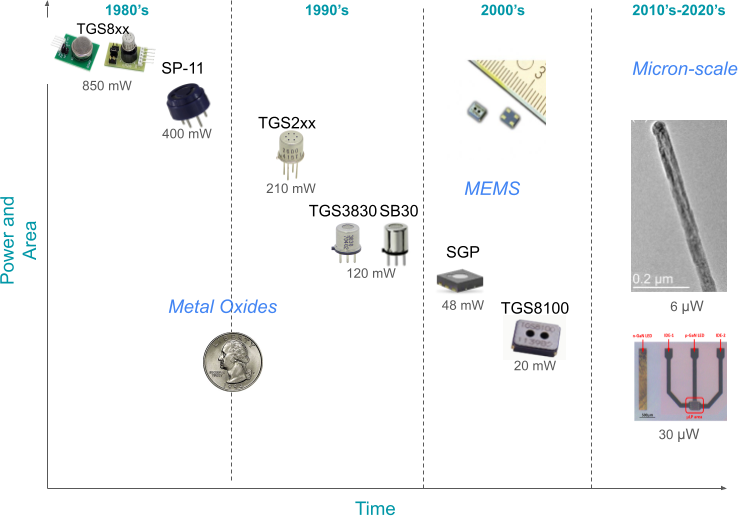
\includegraphics[width=0.7\linewidth]{sensor_timelines.png}
    \caption{\small
        Odor and chemical sensors continue to improve in power, area, and response
        times.
    }
    \label{fig:sensor_timelines}
\end{figure}


Fig.~\ref{fig:sensor_timelines} gives a high-level overview of the
development of chemical sensors used for \olfc{}.  Early sensors, which are
still commercially viable in products such as household smoke detectors, are
both physically large and high powered, as a result of requiring high operating
temperatures (often \(>\SI{500}{\celsius}\)). By greatly reducing the size of
the sensing surface, and thus the power required to heat the surface,
microelectromechanical systems (MEMS) lead to an order of magnitude decrease in
sensor power consumption. However, ultra low-power chemical sensors suitable for
\olfc{} have only come with the development of \si{\micro\meter} scale sensors
in the last decade. Nanowire chemical-resistive sensors enable room-temperature
flexible sensors in the low \si{\micro\watt} power
range~\cite{majhi2021recent}. In fact, recent work has shown self-powered
chemical sensors which exploit the piezoresistive effect of the sensing surface
when it reacts with an analyte~\cite{setiono2019real}. 

As discussed previously, previous work on olfactory processing has largely focused on sensing applications. No prior work addresses
the organization and design of the olfactory processor itself.



\begin{table}[]
\caption{Examples of olfactory applications and their constraints.}
\label{tab:applications}
\begin{adjustbox}{max width=\linewidth}
\begin{tabular}{@{}ll@{}}
\toprule
\textbf{Application}              & \textbf{Constraints}     \\ \midrule
Food Freshness Monitoring         & \(\leq\si{\milli\watt}\), lifetime of hours - months \\
Food Spoilage Detection           & \(\leq\si{\milli\watt}\), lifetime of hours - months \\
Personal Hygiene Monitoring       & low \si{\milli\watt}, lifetime of $\leq$ day         \\
Wearable Body Odor Detection      & low \si{\milli\watt}, lifetime of days               \\
Odor Biometric Authentication     & lifetime of months-years                             \\
Odor Biometric Forensics          & field deployable \& single use                       \\
Smart-Bandage infection detection & \(<\si{\milli\watt}\), lifetime of hours - days      \\
Air and water quality monitoring  & \(<\si{\milli\watt}\), lifetime of months - years    \\
Dangerous compound detection      & lifetime of days-years                               \\
Explosive detection               & lifetime of days-years                               \\
Gas Leak Tracing                  & requires spatial dispersed sensors, lifetime of minutes to hours \\
Odor Cancellation                 & requires odor synthesis  \\
Bespoke clothing deoderization    & requires odor synthesis  \\
Olfactory enabled xR              & requires odor synthesis \\
Food \& Scent recommendation      &                          \\
COPD \& Lung Cancer Screening     &                          \\
    \bottomrule
\end{tabular}
\end{adjustbox}
\end{table}


To build 
%programmable
olfactory computing systems, we must understand and analyze
the computational tasks underpinning odor-based applications. To identify a set of computation tasks that may be common across
a variety of odor-based applications, we surveyed 25 papers published in last 10 years on odor-based applications in Table~\ref{tab:applications} - at least one paper on each application was found. We identified the computational task(s) each paper was focused on. We also surveyed 10 odor-based electronic products in last five years and identified the corresponding computational task(s). Finally, we interviewed three olfaction experts and asked them for a list of computational tasks. We then created a list of tasks that appeared in at least two of the above three lists.

The tasks in our finalized list are
odor localization, odor classification, odor authentication, odor similarity,
active odor cancellation, odor pleasantness estimation, and odor demixing.

Odor classification, as the name suggests, is the task associated with
identifying the source of an odor.  Odor classification uses machine learning
and statistical techniques to map chemical sensor readings to source
odorants~\cite{kaeppler2013odor, husni2017odor}. Odor classification has many
commercial, industrial, agricultural, medical, and security applications,
including food and beverage monitoring for spoilage and quality 
%Assessed goods
%include 
%(e.g., teas
~\cite{yu2008quality, pan2014early},
%chen2013classification, yu2008identification,
%yu2009identification},
%alcohol~\cite{
%zhang2021channel,buratti2004characterization,shi2019deep
%},
%fruits~\cite{pan2014early, chen2018characterization, chen2018development,
%du2019ripeness, rasekh2021nose, %wu2017sensor}, cooking
%oils~\cite{karami2020application, teixeira2021application,
%rasekh2021classification}, meats and seafood~\cite{panigrahi2006design,
%wijaya2019noise, wijaya2021dwtlstm, aunsa2021electronic, grassi2022seafood},
%dairy~\cite{yang2021application, %labreche2005shelf}, and
%vinegar~\cite{li2022physicochemical, anklam1998characterisation}),
%. Industrial
%applications include
%\fi
environmental monitoring for air quality and air pollution
estimation~\cite{caron2019identification, szulczynski2017different,
tacstan2019real, de2008tinynose}, 
%while agriculture applications include
waste-water monitoring and forestry applications~\cite{wilson2013diverse,
blanco2018development, lagod2019application, dewettinck2001electronic},
%. Medical
%applications for odor classification have begun to emerge, including 
hygiene
monitoring~\cite{lorwongtragool2014novel}, diagnosis of lung diseases such
as COPD and lung cancer~\cite{gardner2000electronic, va2021noninvasive,
binson2021discrimination, d2010investigation},
%.  Security applications include
and explosive device detection~\cite{brudzewski2012metal, lopez2017electronic,
sun2013liquid}. Odor classification is performed with a variety of machine
learning and statistical analysis techniques such as principal component
analysis (PCA), support vector machines (SVM), artificial neural networks
(ANN), and K-Means cluster analysis (KMeans).

Biometric authentication using odor, or, odor authentication, is the olfactory
equivalent of fingerprint, facial, iris, or voice authentication techniques
which are currently in vogue on mobile devices~\cite{stokkenes2016biometric}.
Individual humans have an identifiable scent due to genetic and environmental
factors~\cite{penn2007individual}, and many studies have shown successful
discrimination of individuals' body odor using chemical sensor
data~\cite{wongchoosuk2009detection, jha2015quick, jha2016gc}. Several odor
authentication schemes have been proposed~\cite{yang2018human,
shu2014identification}. Odor authentication is similar to odor classification
in that it uses machine learning to classify a body odor as authenticated or
non-authenticated, however, it typically uses a dictionary of known odors.
Similar to other biometric authentication techniques, odor authentication
consists of first extracting features from chemical sensor data, often using
parametric machine learning learning techniques, and then comparing those
features to a user dictionary. Thus, new authenticated users can be enrolled
and old users removed without needing to retrain a new model from the ground
up~\cite{wong2001enhanced}. Algorithms in odor authentication include PCA, SVM,
ANN, K-Means, and KNN.

In the odor similarity task, the goal is to estimate the odor similarity of two
different chemical mixtures.  Traditionally, this has been done by first
identifying the chemical structure of the mixtures' constituent chemicals via
\gcms{}\footnote{However, it can also be done with sensor data}.  These
chemical structures are then mapped to fixed length vectors from an inner
product space, and then the mixtures are represented by weighted sums of the
constituent chemical vectors.  Finally, the similarity of the two chemicals is
scored based on the angle between the two vectors
(AngleDist)~\cite{snitz2013predicting}. %Odor similarity can power an odor
%recommendation engine, in which a new odor is suggested to users based on
%similarity to a known odor the user finds pleasant.

Active odor cancellation is the olfactory equivalent of active noise
cancellation.  Active odor cancellation attempts to `block out' one or more
malodors in an environment by \textit{adding} odors which cancel the malodor,
rendering it as olfactory white noise~\cite{varshney2014active}.
The algorithm which determines how much of each odor to add to the environment
consists of solving a quadratic program which, in many cases, is convex. As
such, gradient descent based optimizers may be used to find local, and often,
global solutions to the optimization problem.

The pleasantness of an odor is highly dependent on the physical properties of
the odorant molecular structure~\cite{arshamian2022perception}. As such, odor
pleasantness estimation is assigning a value (either numeric or categorical) to
a chemical corresponding to its predicted pleasantness.  This has been achieved
using PCA and SVM~\cite{li2018accurate, li2020perception, shang2017machine}.

Odorants exist in mixtures, including time-evolving mixtures, yet often only
one chemical odorant is of interest.  Odor demixing is the task which isolates
the signal corresponding to the chemical of interest.  
This can be achieved
using \gcms{}, however, as \gcms{} requires a large laboratory set-up, and
takes twenty or more minutes to perform. %different techniques are required when
%working with low-power chemical sensors. 
There have been a number of works
which attempt to tackle this problem in context of low-power chemical sensors~\cite{maho2021real, victor2014combining,
fonollosa2014chemical}, but odor demixing remains a largely unexplored \olfc{}
task. However, odor demixing has been studied in biological olfactory systems,
and several studies have proposed biology inspired compressive sensing, which
enables reconstructing sparse signals from many fewer samples than is typically
required (e.g., in an audio setting, from samples taken below the Nyquist
rate)~\cite{fornasier2015compressive}. Compressive sensing, namely, orthogonal
matching pursuit (OMP), has been shown to be useful in the olfactory domain
since individual odors are sparse within the large space in which an odor can
be represented.

Odor localization is the task of identifying the source location of an
odorant `plume' within an environment.  Odor localization is efforts are
exacerbated by the turbulent nature gas plumes which result in non-convex
distributions of the odarant plume with local maxima, which limit the
applicability of gradient based methods.  As such, biology inspired methods, as
well as probabilistic methods such as particle filtering are commonly used in
conjunction with a model of plume dynamics~\cite{vickers2000mechanisms}.
While odor localization
%is unique
%among the tasks in that it 
is typically performed by either a mobile field robot~\cite{chen2019odor}, or
by a distributed sensor network~\cite{hayes2002distributed}, as odor
localization benefits from taking chemical readings in multiple locations
throughout the environment, we also consider future applications where a
wearable aids a moving human or an animal in identifying an odor source (gas
leak or fire source, for example).
%Analogously, consider triangulating a radio signal broadcast
%location --- this task is much easier with receivers in multiple locations than
%with only a single radio receiver.  Indeed, with only a single, fixed chemical
%sensor, it is exceedingly difficult to determine if a faint signal is due
%to a strong odorant source far away, or a weak odorant source nearby.


%\subsection{Algorithms}

 
We will implement the above tasks as a bona fide olfactory computing benchmark suite --- OlfacSuite --- by
    porting all benchmark code to C and OpenMP, designing representative inputs
    for each benchmark, and providing baselines on existing systems. OlfacSuite --- software, data, \& build scripts --- as well as
    executable binaries for major platforms --- will be published under
    an open source license in order to enable commercial and academic
    research into olfactory computing.Data and inputs will be drawn from published real
    world samples.
    
    OlfacSuite will be published with a CMake based build system.  As CMake
    is an open-source, cross platform build automation tool targeting all
    major operating systems, and since nearly all computer architectures
    have open source or proprietary C compilers, researchers will be able
    to get OlfacSuite running on a wide variety of systems quickly and easily.
    For major architectures (e.g., ARMv7, ARMv8, x86\_64, i686, etc.),
    we will provide prebuilt OlfacSuite binaries.



\begin{figure}
    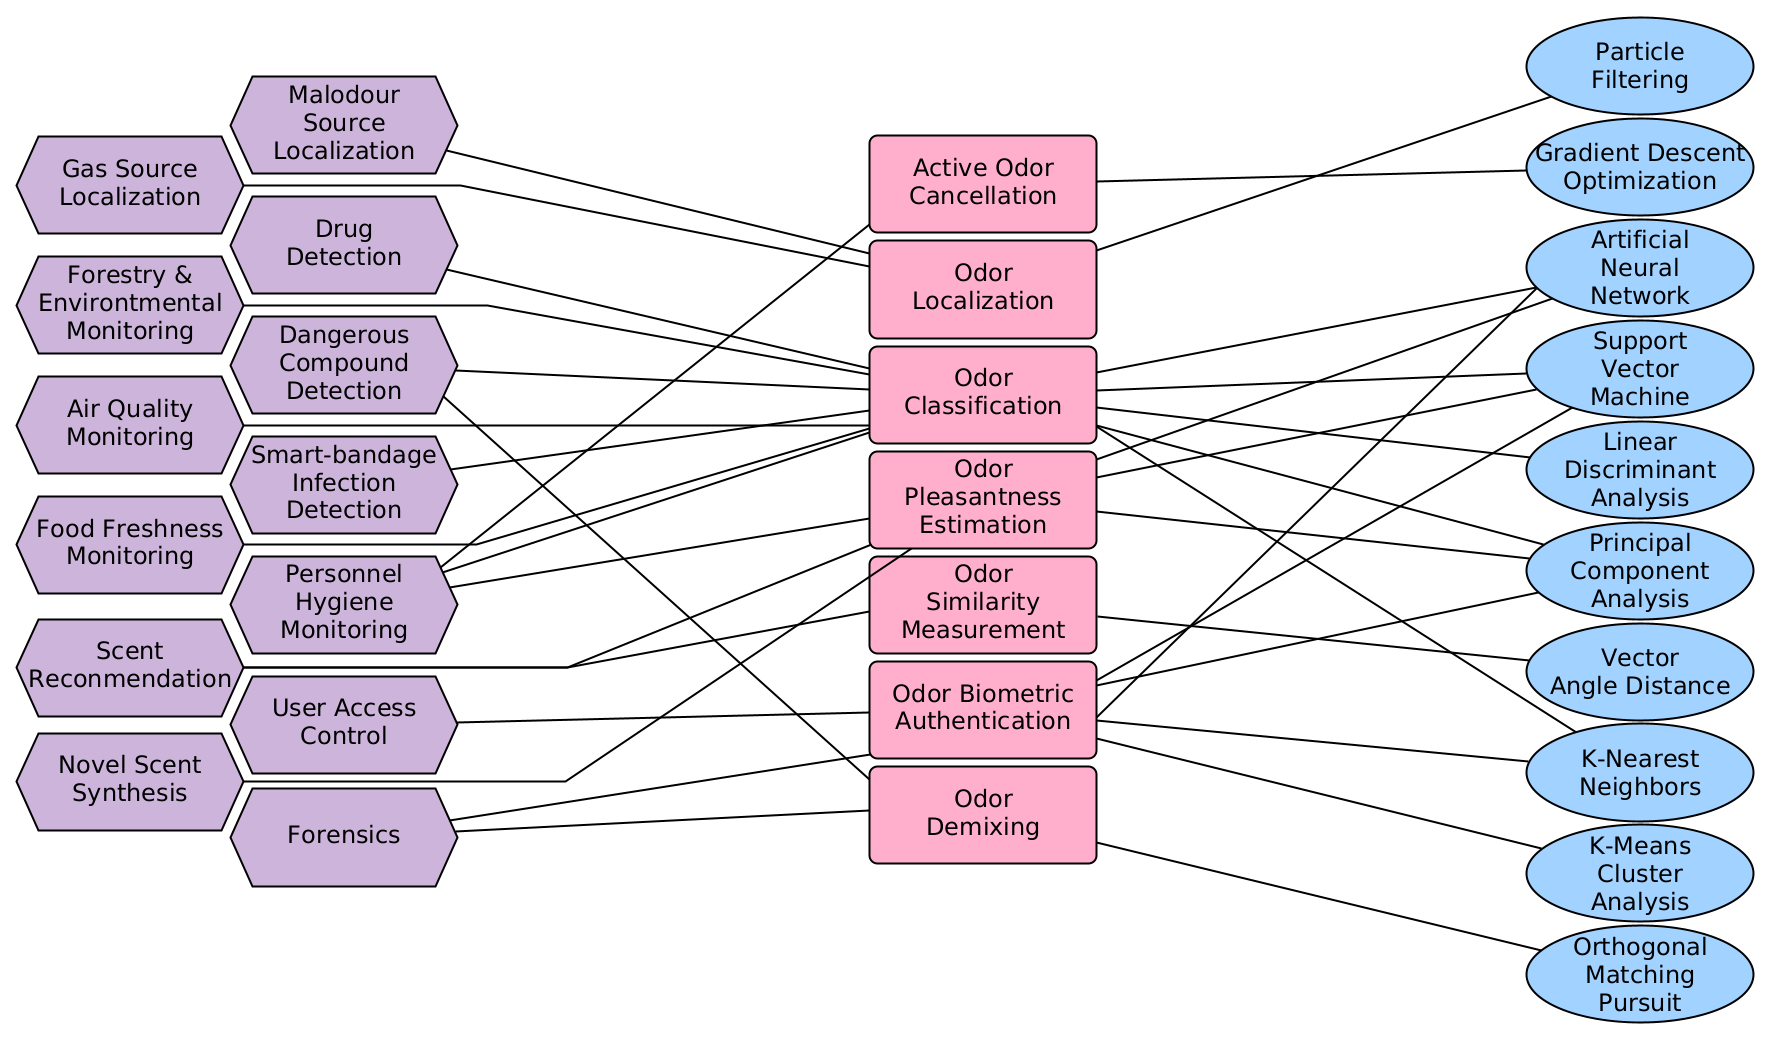
\includegraphics[width=\linewidth]{app_task_kernel.png}
    \caption{
        \small Graphical depiction of relationship between applications
        (\textcolor{purple}{hexagons}) which are composed from tasks
        (\textcolor{pink}{rectangles}).  Tasks are implemented using a
        computational kernel (\textcolor{blue}{ellipses}). Some tasks can be
        supported by multiple kernels.
    }
    \label{fig:app_task_kernel}
\end{figure}

% \input{tables/applications}

To analyze a computer architecture's performance on olfactory workloads, a
diverse and representative collection of olfactory algorithms underpinning the
odor computational tasks is needed.  Fig.~\ref{fig:app_task_kernel} is a graphical depiction of the relationship
between olfactory applications (hexagons), the tasks (ellipses) from which the
applications are composed, and the computational kernels (rectangles) which can
be used to implement the task.  Some tasks may be implemented using one of
several kernels, such as odor classification which can be supported by several
machine learning and statistical analysis techniques. 
%Below we describe the nuances of implementation of the
%identified computational kernels in context
%of \olfc{}.

The algorithms themselves may have olfaction-specific implementation and input characteristics.
For example, particle filtering may require a dynamical model of the
odorant plume.  
Due to the slow rate at which odorant mixtures change,
the number of data points, $d$, in the Principal component analysis for olfactory
applications is limited to the low hundreds,
while the number of sensors in a sensor array is often less than ten.
Thus PCA requires normalizing only a small number of distributions with
a small number of samples, and performing eigen decomposition on a small
correlation matrix.  Similarly, in the odor context, finding the
principal components of an sensed input requires only multiplying the input
by a small $n\times n$ matrix.
Linear discriminant analysis for olfactory applications is extremely light weight,
with time and space complexity quadratic  and linear, respectively,
in the number of sensors in the sensor array.
In olfactory computing, the input
sample is a vector of sensed values from the chemical sensor array. Thus, the
complexity of running the support vector machine is the same as computing the
principal components or linear discrimnants of the input.  
The most prominent type of Artificial neural networks (ANN) seen in olfactory computing is the multilayer
perceptron (MLP), in which each layer is fully connected. The input to the
MLP is typically the sensed data directly, with no preprocessing steps
involved (consider, for example, that there is no need for pre-processing
to help the model learn high-frequency content, as there is in image and audio
processing, since odor signals typically lack high frequency content).
The MLPs used in \olfc{} tend to be just barely deep - often with
only a single hidden layer - and with very few neurons (often $< 50$).
Termination of Kmeans algorithm is known to be NP-Hard~\cite{aloise2009np}.  In practice,
for odor processing, KMeans often terminates quickly~\cite{yang2018human,
zheng2019wearable}.




    
\item
    Rapid development of small and ultra-low power odor sensors means that, for
    the first time, computing power consumption may be the limiting factor
    in olfactory or chemical processing, rather than sensor power
    consumption.  In light of this development, we will perform an exploration
    of the architectural design space in order to identify good architectures
    for \olfc{} systems targeting wearable and distributed sensor networking
    olfactory applications.  Many ultra-low power candidate architectures
    currently exist, including ultra-low power microcontrollers~\cite{} and GPUs~\cite{},
    as well as \(<\si{\milli\watt}\) spatial architectures~\cite{}.
    Preliminary results analyzing olfactory applications
    and their computational requirements (Sec~\ref{ssec:prelim2}) show that,
    for many applications, performance requirements are lax, and absolute
    computational and memory requirements are low.  This suggests that the
    architectural design space considered must go beyond looking at just
    computer organization and design, but must encompass memory design and
    operating points.

    Due to lax performance requirements and low computational requirements,
    \olfc{} is likely a strong candidate for near or sub-threshold
    computing~\cite{}.  Thus the design space exploration will include
    ammenability to and impact of voltage scaling into the near and sub-threshold
    regions.  Although this type of work has been done for CPU and GPU based
    architectures, it has, to the best of our knowledge, never been done for
    reconfigurable spatial architectures.
    
    As many \olfc{} applications require very small amounts of data memory,
        memory design will be an important aspect of the design space
        exploration.  The size, geometry, and number of SRAM banks will be
        explored.  Additionally, since some applications require trivial
        amounts of data memory, we will also consider memories composed wholy
        or partially out of latches and flip-flops, rather than SRAM cells.
        Although SRAM cells are typically smaller and consume less power than
        flip-flops and latches at nominal voltage, SRAM cells are generally not
        ammenable to voltage scaling.  Thus, at low voltages, latch and
        flip-flop based memories may consume less power than an equivalently
        sized SRAM.

\item Analyze Ahromaa and existing olfactory computing hardware in a heterogeneous, networked
     computational setting, in which computation can be offloaded from the earable
     device onto a number of other devices, including smart watches, smart phones,
     and high perfromance cloud systems;


